\clearpage
\setcounter{page}{1}

\begin{center}
\title{\LARGE \bf Chapter 2}\\
\title{\LARGE \bf Pemrograman Dasar}\\
\end{center}

\appendix
\section{Teori}

\begin{enumerate}
\item Variabel

Variabel : tempat penyimpanan sementara untuk data yg berupa integer, boolean, string, array, dan float
Cara penggunaannya : 
1. tidak boleh diawali dengan "\textunderscore" 
2. tidak boleh menggunakan keyword yang sudah ada.
3. variabel bersifat case sensitive

Contoh :
"nama\textunderscore Variabel = data"

\item Operator Aritmatika\\
\begin{tabular}{|c|c|}
\hline
Operator & Simbol\\
\hline
Pembagian & /\\
\hline
Perkalian & *\\
\hline
Penjumlahan & +\\
\hline
Pengurangan & -\\
\hline
Modulus & \% \\
\hline
Pangkat & **\\
\hline
\end{tabular}

Mengubah string ke integer : type data string harus dilakukan casting dengan "int(variable)".
Mengubah integer ke string : type data integer harus dilakukan casting dengan "str(variable)".

\item Syntax Perulangan
\begin{enumerate}[label=\alph*.]
\item While\\ 
While : untuk melakukan looping yang tidak pasti\\
Contoh :\\
i = 0\\
while True :\\
    if i < 100:\\
        print ("i bernilai : "), i\\
        i = i + 1\\
    elif i >= 100:\\
        break\\
\item For\\
For : untuk melakukan looping yang sudah jelas jumlahnya\\
Contoh :\\
for i in range(0, 100):\\
    print (i)\\
\end{enumerate}

\item Syntax Kondisi\\
\begin{enumerate}[label=\alph*.]
\item If\\
If : digunakan untuk percabangan\\
Contoh :\\
umur = 20\\
if umur > 18:\\
    print("wah sudah dewasa")\\
\item Else\\
Else : jika kondisi if tidak terpenuhi maka yang dijalankan kondisi else\\
Contoh :\\
umur = 5\\
if umur > 18:\\
    print ("udah gede ya")\\
else:\\
    print ("masih bayi u")\\
\item Elif\\
Elif : jika kondisi yang didefinisikan cukup banyak, maka menggunakan kondisi elif\\
Contoh :\\
umur = 20\\
if umur > 18 and umur < 30:\\
    print("wah sudah dewasa")\\
elif umur > 30 and umur < 45:\\
    print("masa masa emas")\\
elif umur > 45 and umur < 55:\\
    print("paruh baya")\\
elif umur > 55:\\
    print("masa manula")\\
else:\\
    print("masih kecil ya")\\
\end{enumerate}

\item Error\\
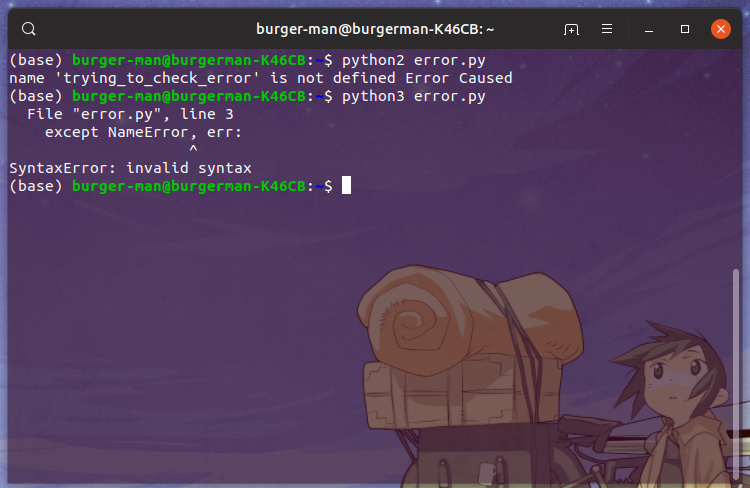
\includegraphics{gambar/error.png}
pada kodingan harus diberikan indentasi 

\item Try Except\\
Try except : salah satu penanganan error\\
Contoh :\\
try:\\
	x = 1/0\\
except Exception, e:\\
	print e\\

print(x+1)
\end{enumerate}

\section{Keterampilan Pemrograman}

\begin{enumerate}

\item
\lstinputlisting[language=Python]{src/NPM(1).py}

\item
\lstinputlisting[language=Python]{src/NPM(2).py}

\item
\lstinputlisting[language=Python]{src/NPM(3).py}

\item
\lstinputlisting[language=Python]{src/NPM(4).py}

\item
\lstinputlisting[language=Python]{src/NPM(5).py}

\item
\lstinputlisting[language=Python]{src/NPM(6).py}

\item
\lstinputlisting[language=Python]{src/NPM(7).py}

\item
\lstinputlisting[language=Python]{src/NPM(8).py}

\item
\lstinputlisting[language=Python]{src/NPM(9).py}

\item
\lstinputlisting[language=Python]{src/NPM(10).py}

\item
\lstinputlisting[language=Python]{src/NPM(11).py}

\end{enumerate}

\section{Keterampilan Penanganan Error}
\begin{enumerate}
\item Peringatan error\\

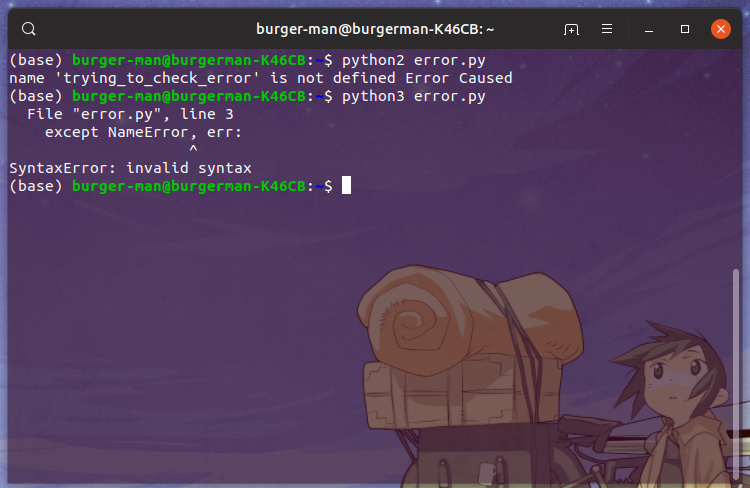
\includegraphics{gambar/error.png}
Penanganan Error dengan menambahkan indentasi.

\item Try Except\\
\lstinputlisting[language=Python]{src/2err.py}
\end{enumerate}
